\documentclass[a4paper&11pt]{article}
\usepackage{caption}
\usepackage{subcaption}
\usepackage{float}
\usepackage[caption = false]{subfig}
\usepackage{graphicx}

\newcommand{\subf}[2]{%
  {\small\begin{tabular}[t]{@{}c@{}}
  #1\\#2
  \end{tabular}}%
}  


\begin{document}
\section*{Simulation 1}

\subsection*{Graphs, subgraph and Edge Probability - Diameter}

\subsubsection*{Erdos-Renyi Graphs}


\begin{table}[H]
\centering

\label{my-label}
\resizebox{\textwidth}{!}{\begin{tabular}{c|c|c|c|c|c|c|c|c}
\hline
index & pn & order & size & density & cluster coefficient &diameter & nodes deg $\geq$ n & largest component \\ \hline
0& 1& 143& 117& 0.011523687580025609& 0.0& inf& 0& 97\\ \hline
1& 3& 143& 325& 0.032010243277848911& 0.03655788655788656& 7& 0& 143\\ \hline
2& 5& 143& 527& 0.051905840638235001& 0.05108083447244284& 5& 14& 143\\ \hline
3& 7& 143& 757& 0.074559243573328077& 0.0733257571774318& 4& 49& 143\\ \hline
4& 9& 143& 885& 0.087166354771988572& 0.08693534635371428& 4& 87& 143\\ \hline
5& 11& 143& 1111& 0.10942578548212351& 0.1088499366852766& 3& 128& 143\\ \hline


\end{tabular}}

\caption{Simulation 1: Graph properties for different probabilities $pn$ of edge existence between nodes in Erdos-Renyi graphs }
\end{table}



\begin{figure}[H]
\centering
\begin{tabular}{|c|c|}
\hline
\subf{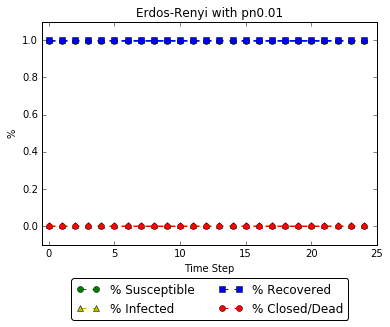
\includegraphics[width=60mm]{ploter01.png}}
     {}
&
\subf{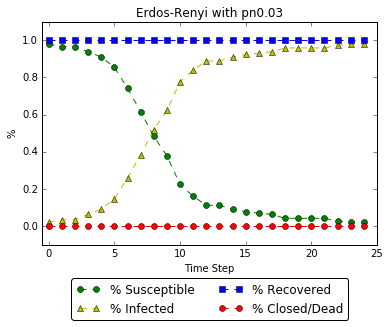
\includegraphics[width=60mm]{ploter03.png}}
     {}
\\
\hline
\subf{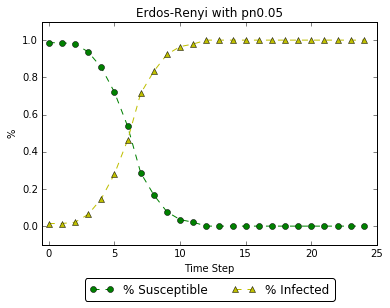
\includegraphics[width=60mm]{ploter05.png}}
     {}
&
\subf{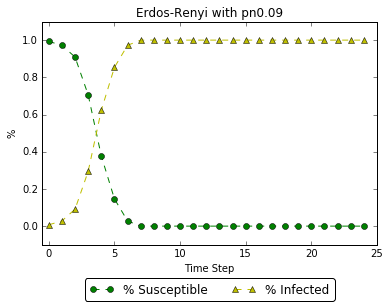
\includegraphics[width=60mm]{ploter09.png}}
     {}
\\
\hline
\end{tabular}
\caption{Simulation 1 Erdos Renyi : Plotting Node States for Graphs for pn = 0.01, 0.03, 0.05, 0.09}
\end{figure}

\subsubsection*{Real Airport Graph and subgraphs}

\begin{table}[H]
\centering

\label{my-label}
\resizebox{\textwidth}{!}{\begin{tabular}{c|c|c|c|c|c|c|c}
\hline
Name & order & size & density & cluster coefficient &diameter & nodes deg $\geq$ n & largest component\\ \hline
Real World Graph & 143& 1452& 0.14301191765980498& 0.6410089238208931& 4& 73& 143\\ \hline
Largest Edge Weights &13 & 10 & 0.12820512820512819& 0.0 & inf &1& 7\\ \hline
Lowest Edge Weights & 27 & 102 & 0.29059829059829062 & 0.6458430700260764& 3& 13& 27\\ \hline
20 Largest Deg. Cent. & 20& 177& 0.93157894736842106& 0.9423609156581293& 2& 20& 20\\ \hline
Min Span. Tree & 143& 142& 0.013986013986013986& 0.0& 8& 3& 143\\ \hline
\end{tabular}}
\caption{Real World Airport graph and subgraphs graph properties}
\end{table}

\begin{center}
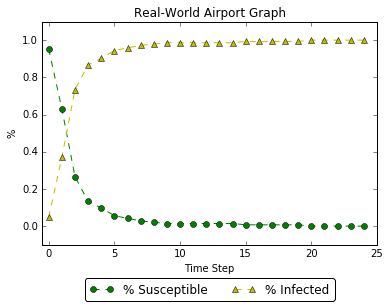
\includegraphics[scale=0.8]{realworldplot.png}
\begin{figure}[H]
\caption{Simulation 1 Real-world :  Airports graph properties}
\end{figure}
\end{center}


\begin{figure}[H]
\centering
\begin{tabular}{|c|c|}
\hline
\subf{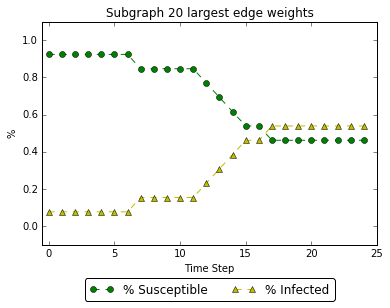
\includegraphics[width=60mm]{sublargedgewsim1.png}}
     {}
&
\subf{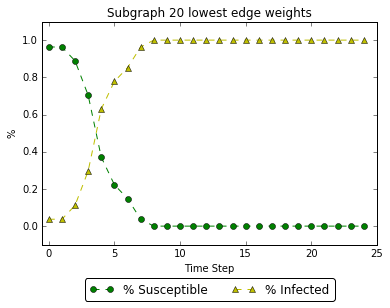
\includegraphics[width=60mm]{sublowestedgewsim1.png}}
     {}
\\
\hline
\subf{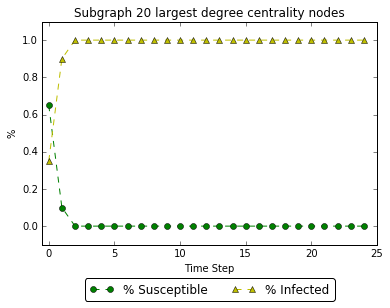
\includegraphics[width=60mm]{largestdegcsim1.png}}
     {}
&
\subf{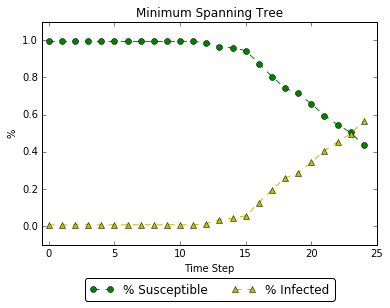
\includegraphics[width=60mm]{minspansim1.png}}
     {}
\\
\hline
\end{tabular}
\caption{Simulation 1  Real-world : Subgraph node state plots}
\end{figure}

\subsection*{Source Node Centrality}
\subsubsection*{Erdos-Renyi Graph with p = 0.09}


%Begin: Sim1 - generated
\begin{figure}[H]
\centering
\begin{tabular}{|c|c|}
\hline
\subf{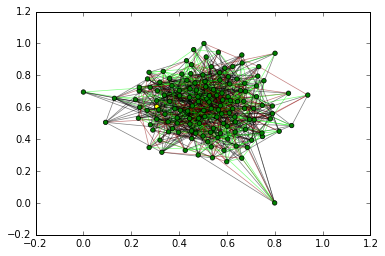
\includegraphics[width=60mm]{21InitialNode_Center_of_graph_1.png}}
     {}
&
\subf{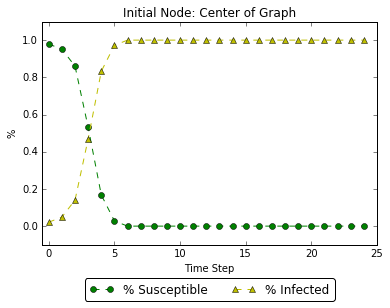
\includegraphics[width=60mm]{21InitialNode_Center_of_graph_2.png}}
     {}
\\
\hline
\end{tabular}
\caption{Simulation 1 Erdos-Renyi : Initial Node Center Of Graph}
\end{figure}



\begin{figure}[H]
\centering
\begin{tabular}{|c|c|}
\hline
\subf{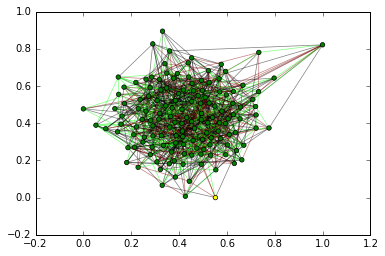
\includegraphics[width=60mm]{21MinDegree_Centrality_source_node_1.png}}
     {}
&
\subf{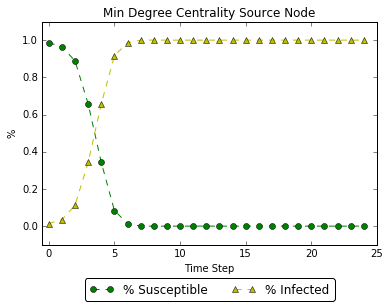
\includegraphics[width=60mm]{21MinDegree_Centrality_source_node_2.png}}
     {}
\\
\hline
\subf{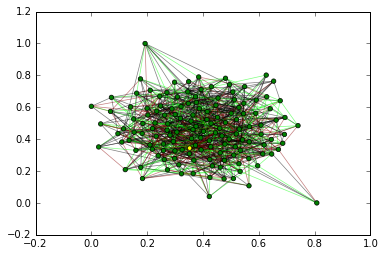
\includegraphics[width=60mm]{21MaxDegree_Centrality_source_node_1.png}}
     {}
&
\subf{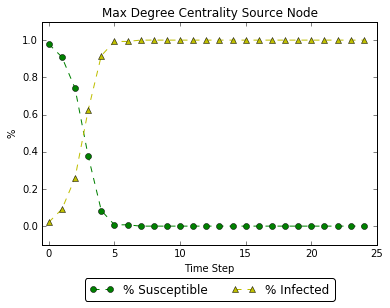
\includegraphics[width=60mm]{21MaxDegree_Centrality_source_node_2.png}}
     {}
\\
\hline
\end{tabular}
\caption{Simulation 1 Erdos-Renyi : Max and Min Degree Centrality SourceNode}
\end{figure}


\begin{figure}[H]
\centering
\begin{tabular}{|c|c|}
\hline
\subf{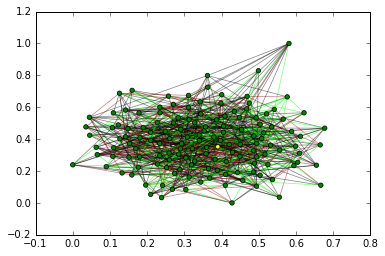
\includegraphics[width=60mm]{21MaxBetweeness_centrality_sourcenode_1.png}}
     {}
&
\subf{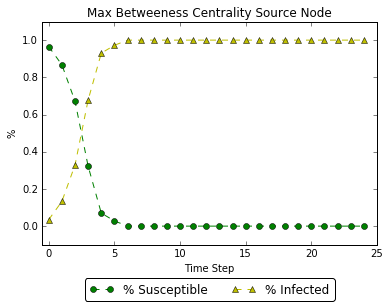
\includegraphics[width=60mm]{21MaxBetweeness_centrality_sourcenode_2.png}}
     {}
\\
\hline
\subf{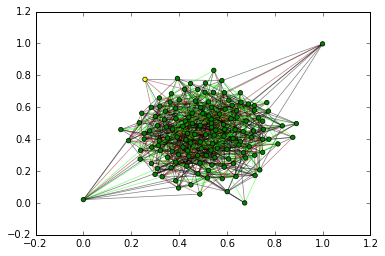
\includegraphics[width=60mm]{21MinBetweeness_centrality_sourcenode_1.png}}
     {}
&
\subf{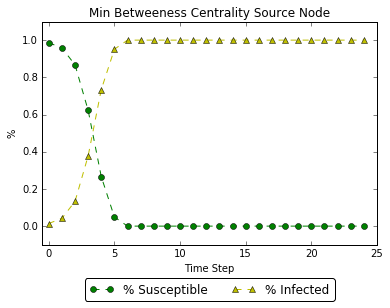
\includegraphics[width=60mm]{21MinBetweeness_centrality_sourcenode_2.png}}
     {}
\\
\hline
\end{tabular}
\caption{Simulation 1 Erdos-Renyi : Max and Min Betweenness Centrality SourceNode}
\end{figure}

%End: Sim1 - generated






\subsubsection*{Real World Graph}

%
%Begin: Sim1 - Real 

\begin{figure}[H]
\centering
\begin{tabular}{|c|c|}
\hline
\subf{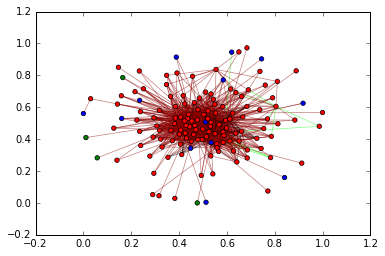
\includegraphics[width=60mm]{11InitialNode_Center_of_graph_1.png}}
     {}
&
\subf{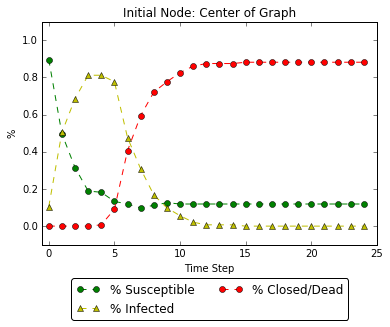
\includegraphics[width=60mm]{11InitialNode_Center_of_graph_2.png}}
     {}
\\
\hline
\end{tabular}
\caption{Simulation 1 Real : Initial Node Center Of Graphe}
\end{figure}


\begin{figure}[H]
\centering
\begin{tabular}{|c|c|}
\hline
\subf{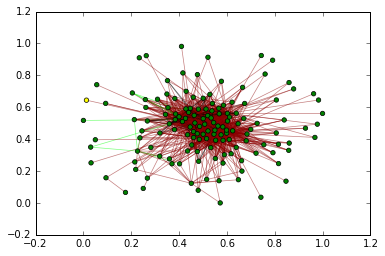
\includegraphics[width=60mm]{11MinDegree_Centrality_source_node_1.png}}
     {}
&
\subf{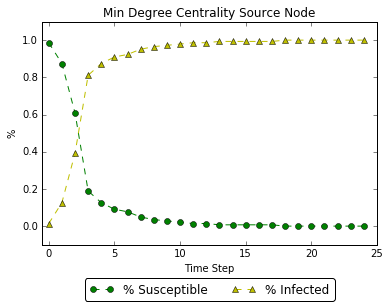
\includegraphics[width=60mm]{11MinDegree_Centrality_source_node_2.png}}
     {}
\\
\hline
\subf{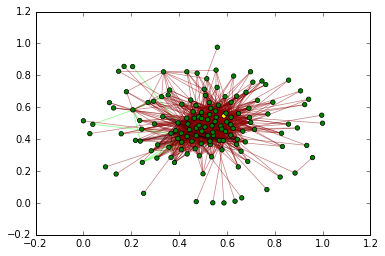
\includegraphics[width=60mm]{11MaxDegree_Centrality_source_node_1.png}}
     {}
&
\subf{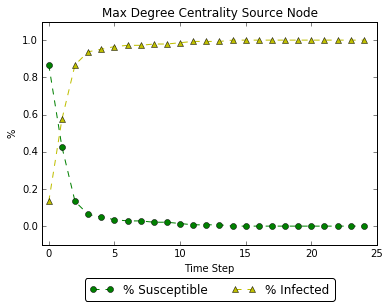
\includegraphics[width=60mm]{11MaxDegree_Centrality_source_node_2.png}}
     {}
\\
\hline
\end{tabular}
\caption{Simulation 1 Real : Max and Min Degree Centrality SourceNode}
\end{figure}


\begin{figure}[H]
\centering
\begin{tabular}{|c|c|}
\hline
\subf{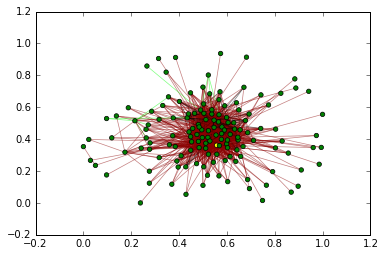
\includegraphics[width=60mm]{11MaxBetweeness_centrality_sourcenode_1.png}}
     {}
&
\subf{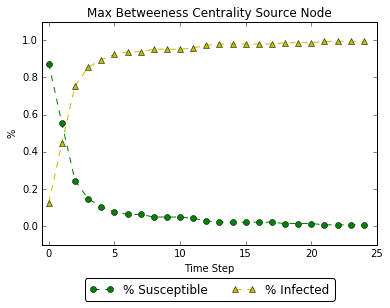
\includegraphics[width=60mm]{11MaxBetweeness_centrality_sourcenode_2.png}}
     {}
\\
\hline
\subf{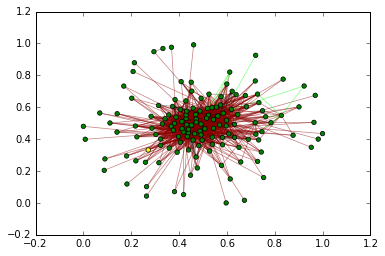
\includegraphics[width=60mm]{11MinBetweeness_centrality_sourcenode_1.png}}
     {}
&
\subf{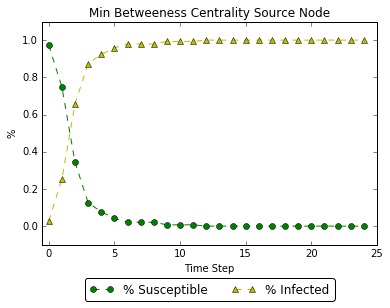
\includegraphics[width=60mm]{11MinBetweeness_centrality_sourcenode_2.png}}
     {}
\\
\hline
\end{tabular}
\caption{Simulation 1 Real : Max and Min Betweenness Centrality SourceNode}
\end{figure}

%End: Sim1 - Real 

\section*{Simulation 2}
\subsection*{Erdos-Renyi Graphs}


\begin{table}[H]
\centering

\label{my-label}
\resizebox{\textwidth}{!}{\begin{tabular}{c|c|c|c|c|c|c|c|c}
\hline
index & pn & order & size & density & cluster coefficient &diameter & nodes deg $\geq$ n & largest component\\ \hline
0& 1& 143& 103& 0.010144784792672116& 0.008857808857808859& inf& 0& 81\\ \hline
 1& 3& 143& 310& 0.030532847434255887& 0.017199467199467203& inf& 0& 141\\ \hline
 2& 5& 143& 530& 0.052201319806953611& 0.045021276314982595& 5& 12& 143\\ \hline
 3& 7& 143& 734& 0.072293903279818772& 0.07440109217101569& 4& 49& 143\\ \hline
 4& 9& 143& 889& 0.087560326996946714& 0.09322985284361361& 4& 86& 143\\ \hline
 5& 11& 143& 1162& 0.1144489313503398& 0.11609641591068731& 3& 128& 143\\ \hline
\end{tabular}}

\caption{Simulation 2 Erdos Renyi :  Graph properties for pn = 0.01, 0.03, 0.05, 0.09}
\end{table}


\begin{figure}[H]
\centering
\begin{tabular}{|c|c|}
\hline
\subf{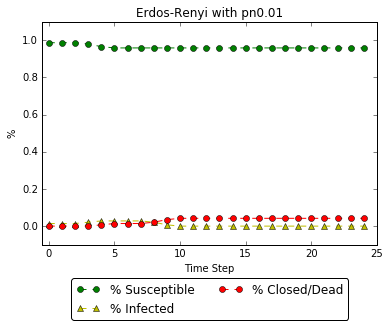
\includegraphics[width=60mm]{plotdie01.png}}
     {}
&
\subf{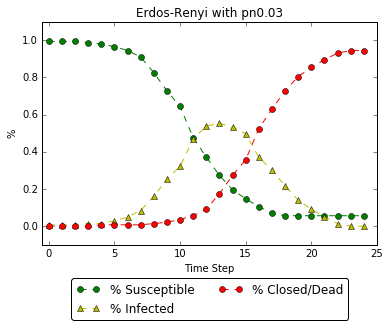
\includegraphics[width=60mm]{plotdie03.png}}
     {}
\\
\hline
\subf{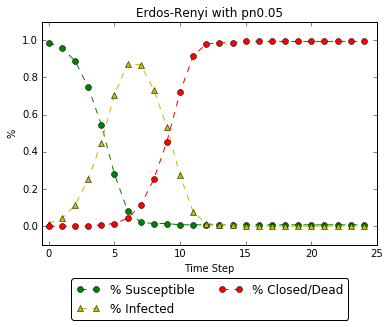
\includegraphics[width=60mm]{plotdie05.png}}
     {}
&
\subf{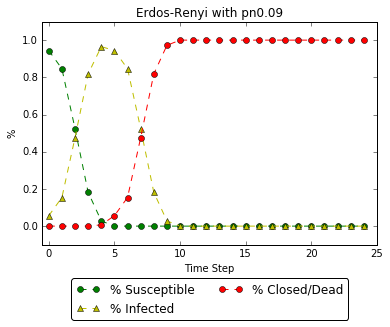
\includegraphics[width=60mm]{plotdie09.png}}
     {}
\\
\hline
\end{tabular}
\caption{Simulation 2 Erdos Renyi :  Plotting Node States for Graphs for pn = 0.01, 0.03, 0.05, 0.09}
\end{figure}

\subsubsection*{Real Airports Graph and subgraphs}




\begin{center}
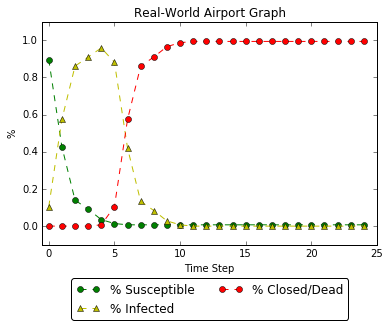
\includegraphics[scale=0.8]{realworldplotsim2.png}
\begin{figure}[H]
\caption{Simulation 2 Real-world :  airport graph properties}
\end{figure}
\end{center}

\begin{figure}[H]
\centering
\begin{tabular}{|c|c|}
\hline
\subf{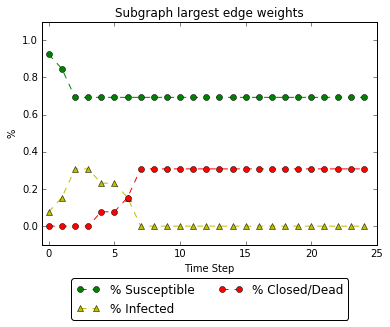
\includegraphics[width=60mm]{largestedgesim2.png}}
     {}
&
\subf{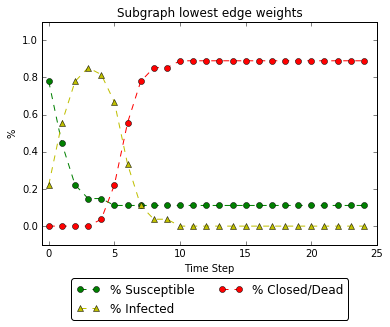
\includegraphics[width=60mm]{lowestedgesim2.png}}
     {}
\\
\hline
\subf{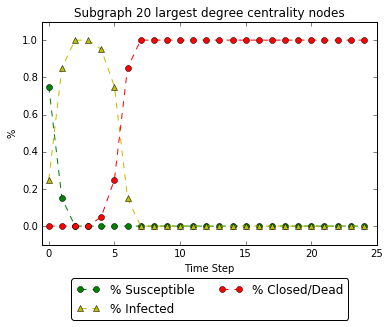
\includegraphics[width=60mm]{largestsim2.png}}
     {}
&
\subf{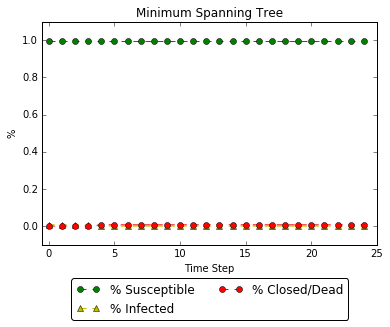
\includegraphics[width=60mm]{minspantreesim2.png}}
     {}
\\
\hline
\end{tabular}
\caption{Simulation 2 Erdos Renyi : Plotting Node States for Graphs for pn = 0.1, 0.3, 0.5, 0.9}
\end{figure}


\subsection*{Source Node Centrality}
\subsubsection*{Erdos-Renyi Graph with p = 0.09}
%Begin: Sim2 - generated 
\begin{figure}[H]
\centering
\begin{tabular}{|c|c|}
\hline
\subf{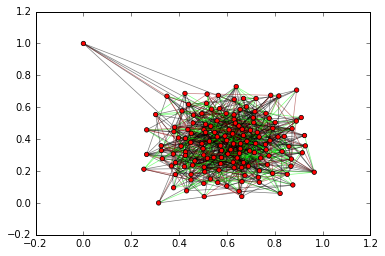
\includegraphics[width=60mm]{22InitialNode_Center_of_graph_1.png}}
     {}
&
\subf{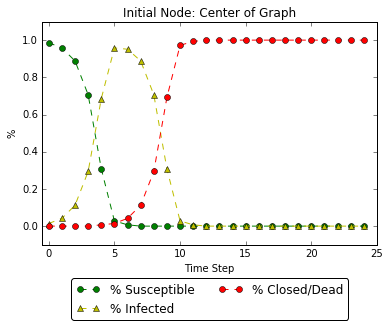
\includegraphics[width=60mm]{22InitialNode_Center_of_graph_2.png}}
     {}
\\
\hline
\end{tabular}
\caption{Simulation 2 Erdos-Renyi : Initial Node Center Of Graph}
\end{figure}


\begin{figure}[H]
\centering
\begin{tabular}{|c|c|}
\hline
\subf{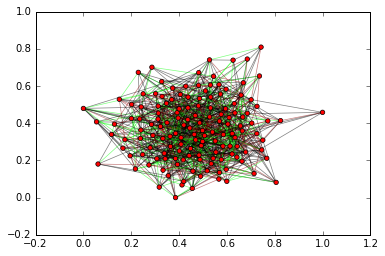
\includegraphics[width=60mm]{22MinDegree_Centrality_source_node_1.png}}
     {}
&
\subf{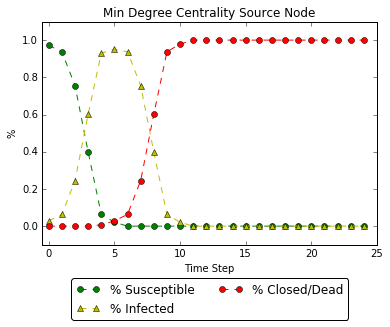
\includegraphics[width=60mm]{22MinDegree_Centrality_source_node_2.png}}
     {}
\\
\hline
\subf{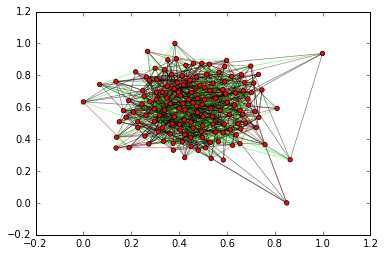
\includegraphics[width=60mm]{22MaxDegree_Centrality_source_node_1.png}}
     {}
&
\subf{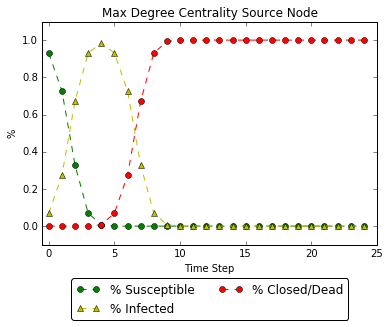
\includegraphics[width=60mm]{22MaxDegree_Centrality_source_node_2.png}}
     {}
\\
\hline
\end{tabular}
\caption{Simulation 2 Erdos-Renyi : Max and Min Degree Centrality SourceNode}
\end{figure}


\begin{figure}[H]
\centering
\begin{tabular}{|c|c|}
\hline
\subf{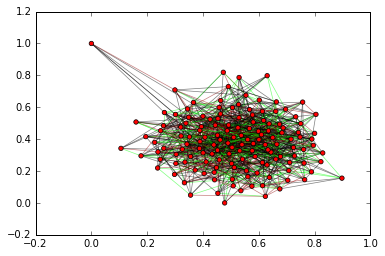
\includegraphics[width=60mm]{22MaxBetweeness_centrality_sourcenode_1.png}}
     {}
&
\subf{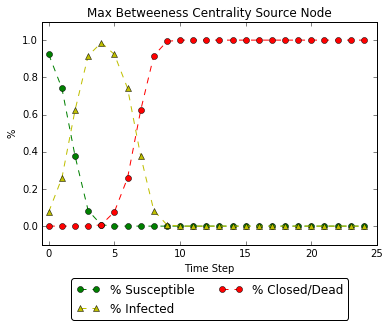
\includegraphics[width=60mm]{22MaxBetweeness_centrality_sourcenode_2.png}}
     {}
\\
\hline
\subf{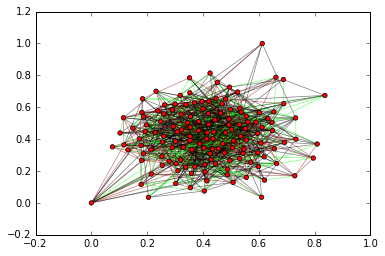
\includegraphics[width=60mm]{22MinBetweeness_centrality_sourcenode_1.png}}
     {}
&
\subf{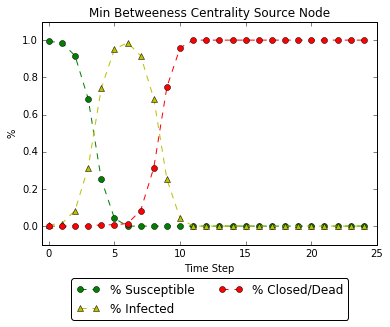
\includegraphics[width=60mm]{22MinBetweeness_centrality_sourcenode_2.png}}
     {}
\\
\hline
\end{tabular}
\caption{Simulation 2 Erdos-Renyi : Max and Min Betweenness Centrality SourceNode}
\end{figure}

%End: Sim2 - generated 

\subsubsection*{Real World Airports Graph}
%Begin: Sim2 - Real 

\begin{figure}[H]
\centering
\begin{tabular}{|c|c|}
\hline
\subf{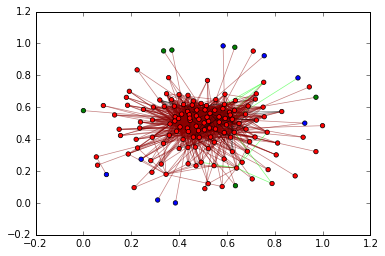
\includegraphics[width=60mm]{InitialNode_Center_of_graph_1.png}}
     {}
&
\subf{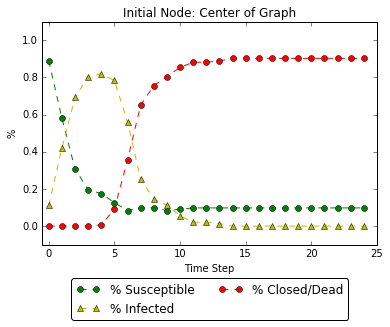
\includegraphics[width=60mm]{InitialNode_Center_of_graph_2.png}}
     {}
\\
\hline
\end{tabular}
\caption{Simulation 2 Real : Initial Node Center Of Graph}
\end{figure}



\begin{figure}[H]
\centering
\begin{tabular}{|c|c|}
\hline
\subf{\includegraphics[width=60mm]{MinDegree_Centrality_source_node_1.png}}
     {}
&
\subf{\includegraphics[width=60mm]{MinDegree_Centrality_source_node_2.png}}
     {}
\\
\hline
\subf{\includegraphics[width=60mm]{MaxDegree_Centrality_source_node_1.png}}
     {}
&
\subf{\includegraphics[width=60mm]{MaxDegree_Centrality_source_node_2.png}}
     {}
\\
\hline
\end{tabular}
\caption{Simulation 2 Real : Max and Min Degree Centrality SourceNode}
\end{figure}


\begin{figure}[H]
\centering
\begin{tabular}{|c|c|}
\hline
\subf{\includegraphics[width=60mm]{MaxBetweeness_centrality_sourcenode_1.png}}
     {}
&
\subf{\includegraphics[width=60mm]{MaxBetweeness_centrality_sourcenode_2.png}}
     {}
\\
\hline
\subf{\includegraphics[width=60mm]{MinBetweeness_centrality_sourcenode_1.png}}
     {}
&
\subf{\includegraphics[width=60mm]{MinBetweeness_centrality_sourcenode_2.png}}
     {}
\\
\hline
\end{tabular}
\caption{Simulation 2 Real : Max and Min Betweenness Centrality SourceNode}
\end{figure}

%End: Sim2 - Real 


\end{document}